%-------------------------------------------------------------------------------
%	PAQUETES Y OTRAS CONFIGURACIONES
%-------------------------------------------------------------------------------

%-------------------------------------------------------------------------------
%	PAQUETES Y OTRAS CONFIGURACIONES
%-------------------------------------------------------------------------------
\documentclass{tufte-handout}
%\documentclass[paper=letter, fontsize=11pt]{scrartcl} % Tamaño de papel y letra para el documento
\usepackage{geometry}
\geometry{left=1.2cm, right=6.2cm, top=2.5cm, bottom=2.5cm}
\usepackage{color}
\usepackage[utf8]{inputenc} % Los caracteres acentuados se pueden escribir normalmente en el código
\usepackage[T1]{fontenc} % Configuración de fuente de salida
\usepackage{cmbright}
\usepackage[sfdefault]{noto}
\usepackage[T1]{fontenc}
\normalfont
\usepackage{graphicx} % Paquetes para incluir imágenes
\usepackage{multicol}
\usepackage{circuitikz}
\usepackage{tikz}
\usetikzlibrary{arrows}

\usepackage{sectsty} % Paquete para configuración de secciones
\allsectionsfont{\centering \normalfont \scshape} % Los títulos de las secciones son centrados, con la misma fuente y pequeñas mayúsculas

\usepackage{todonotes}
\usepackage{microtype}
\renewcommand{\figurename}{Figura}

\usepackage{listings}
\renewcommand{\lstlistingname}{Código}
\lstdefinestyle{mystyle}{
    basicstyle=\footnotesize,
    breakatwhitespace=false,
    breaklines=true,
    captionpos=b,
    keepspaces=true,
    numbers=left,
    numbersep=5pt,
    showspaces=false,
    showstringspaces=false,
    showtabs=false,
    tabsize=2
}
\lstset{style=mystyle}

% \usepackage{fancyhdr} % Paquete para personalizar pies y cabeceras de página
% \pagestyle{fancyplain} % Todas las páginas con las mismas cabeceras y pies de página
% \fancyhead{} % Sin cabecera
% \fancyfoot[L]{} % Vacío en la izquierda del pie de página
% \fancyfoot[C]{} % Vacío en el centro del pie de página
% \fancyfoot[R]{\thepage} % Número de página en el pie de pagina
% \renewcommand{\headrulewidth}{0pt} % Sin lineas en la cabecera
% \renewcommand{\footrulewidth}{0pt} % Sin lineas en el pie de página
% \setlength{\headheight}{13.6pt} % Altura de cabecera
%
% \numberwithin{equation}{section} % Numera ecuaciones en cada sección
% \numberwithin{figure}{section} % Numera figuras en cada sección
% \numberwithin{table}{section} % Numera tablas en cada sección
%
% \setlength\parindent{0pt} % Quita la indentación de los párrafos

\newcommand{\horrule}[1]{\rule{\linewidth}{#1}} % Comando personalizado para hacer linea horizontal


%-------------------------------------------------------------------------------
%	TITULO
%-------------------------------------------------------------------------------

\title{Práctica 5 - Control de servomotores\\Interfaces y periféricos para robots}
\author{Roberto Cadena Vega} % Nombre del profesor
\date{}

%-------------------------------------------------------------------------------
%	EMPIEZA EL DOCUMENTO
%-------------------------------------------------------------------------------

\begin{document}
\maketitle % Imprime el título

%-------------------------------------------------------------------------------
%	OBJETIVOS
%-------------------------------------------------------------------------------

\section{Objetivos}

	Controlar la posición de un motor de corriente directa con un sensor de realimentación (servomotor).

%-------------------------------------------------------------------------------
%	CONOCIMIENTOS PREVIOS
%-------------------------------------------------------------------------------

\section{Conocimientos Previos}

%-------------------------------------------------------------------------------

	\subsection{Controladores}

		%\begin{marginfigure}
		%	\begin{center}
		%		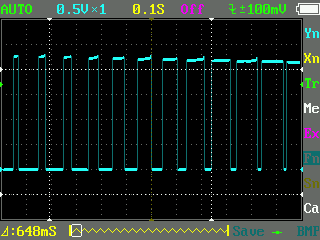
\includegraphics[width=\textwidth]{images/PWM_fade.png}
		%		\caption{PWM variante con el tiempo}
		%		\label{fig:PWM_fade}
		%	\end{center}
		%\end{marginfigure}

		%\begin{figure}
		%	\begin{center}
		%		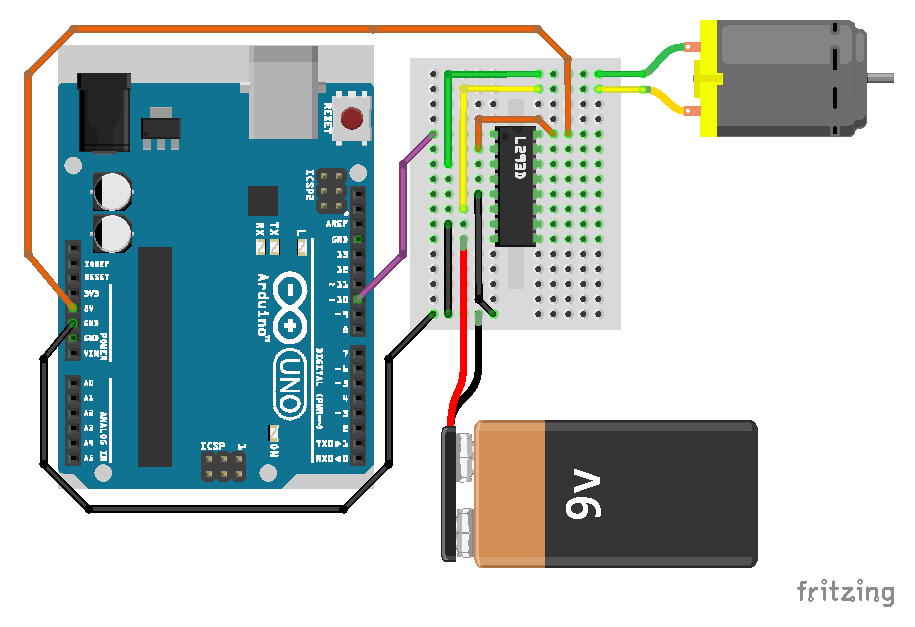
\includegraphics[width=0.8\textwidth]{images/Arduino-L293D-CD.pdf}
		%		\caption{Conexion Arduino - L293D - Motor CD}
		%		\label{fig:motor_arduino}
		%	\end{center}
		%\end{figure}

		%\lstinputlisting[language=C]{codigos/dc_motor_vel.ino}

		En esta práctica utilizaremos primero el servomotor de la manera en que el fabricante esperaba que lo usaramos, despues lo modificaremos de tal manera en que podamos controlarlo completamente desde el Arduino.

		En primer lugar debemos saber como funciona normalmente; para esto lo conectaremos de acuerdo a las instrucciones del fabricante, tomando cuidado de conectar el cable de señal al pin 13 de la tarjeta de desarrollo Arduino, para darle la señal de control por medio de este.

		Ahora podemos subir el siguiente código a nuestro Arduino, con el que podremos modificar su posición por medio de comandos en el monitor serial del IDE de Arduino.

		\lstinputlisting[language=C]{codigos/servo_comercial_serial.ino}

		%\newpage

%-------------------------------------------------------------------------------
%	EQUIPO
%-------------------------------------------------------------------------------

\section{Equipo}

	El siguiente equipo será proporcionado por el laboratorio, siempre y cuando lleguen en los primeros 15 minutos de la práctica, y hagan el vale conteniendo el siguiente equipo (exceptuando las pinzas).

	\begin{itemize}
		\item Fuente de alimentación
		\item Osciloscopio
		\item Cables BNC - Caimán
		\item Cables de alimentación
		\item Multímetro
		\item Pinzas
	\end{itemize}

%-------------------------------------------------------------------------------
%	MATERIALES
%-------------------------------------------------------------------------------

\section{Materiales}

	\begin{itemize}
		\item Protoboard
		\item Cables
		\item Motor CD
		\item LED
		\item ULN2003A, L293D, L298N, etc.
	\end{itemize}

%-------------------------------------------------------------------------------
%	DESARROLLO
%-------------------------------------------------------------------------------

\section{Desarrollo}

	Diseña los circuitos requeridos, el código necesario para que estos funciones y responde las preguntas de la hoja de anotaciones.

%-------------------------------------------------------------------------------
%	CONCLUSIONES
%-------------------------------------------------------------------------------

\section{Conclusiones}
	El alumno deberá describir sus conclusiones al final de su reporte de práctica.

%-------------------------------------------------------------------------------
%	HOJA DE ANOTACIONES
%-------------------------------------------------------------------------------

\clearpage
\section{Hoja de Anotaciones}

	\begin{enumerate}
		\item Diseña el circuito necesario para conectar tu motor al Arduino, utilizando el CI que conseguiste. \\ \vspace{7cm}
		\item Escribe el código necesario para que el motor conectado al Arduino cambie de velocidad, cuando se le envie el duty cycle por medio del monitor serial. \\
		\item Si necesito que el motor gire en el sentido contrario, ¿Que cambio tengo que hacer en el circuito que diseñaste? \\ \vspace{7cm}
		\item Escribe el código necesario para que el motor conectado al Arduino empiece a girar con la velocidad requerida en la instrucción \texttt{M3 S1000}, en donde \texttt{1000} se refiere a $1000rpm$; suponga que el motor trabaja en un rango de velocidades de $0rpm$ a $5000rpm$. El motor debe parar cuando se envia la instrucción \texttt{M5} o \texttt{M3 S0}. Cuando cada instrucción sea ejecutada, el Arduino debe mandar el texto \texttt{ok} por el puerto serial a la computadora.\\
	\end{enumerate}

	\begin{multicols}{2}
		Integrantes del equipo: \\[0.4cm]
		\horrule{0.5pt} \\[0.4cm] % Linea horizontal delgada
		\horrule{0.5pt} % Linea horizontal delgada

		Revisó: \\[1.25cm]
		\horrule{0.5pt} \\% Linea horizontal delgada
	\end{multicols}

%-------------------------------------------------------------------------------
%	FIN DEL DOCUMENTO
%-------------------------------------------------------------------------------

\end{document}
